\chapter{Prostředí FN Plzeň}
\label{ch:fn}

Tato kapitola se zabývá obecným popisem prostředí jednotky intenzivní péče ve FN Plzeň, databáze ve FN Plzeň a aplikace WinMedicalc - karet \emph{Ordinované léky}, \emph{Bilance tekutin} a \emph{Invazivní přístupy}.

\section{Práce zdravotních sester}

Práce zdravotních sester v nemocnici je náročná a vyžaduje zodpovědnost. Sestry musí být pečlivé a nedělat chyby, které by mohly ohrozit zdravotní stav pacienta. Obvzlášť tomu je na jednotkách intenzivní péče, kde musí rychle reagovat na změny stavu pacientů. Tomu musí být přizpůsobená i vyvíjená aplikace. Její ovládání musí být jednoduché a intuitivní, aby práce s ní byla efektivní.

Zdravotní sestry na jednotce intenzivní péče často pracují v latexových rukavicích. Tomu by mělo odpovídat i uživatelské rozhraní. Jednotlivé komponenty by proto měly být dostatečně veliké, aby nedocházelo ke zbytečným překlepům. Je třeba počítat i s tím, že některá zdravotní sestra může mít zrakovou vadu. Neustálé nasazování brýlí by ji poté zdržovalo od práce. Také proto je nutné použít dostatečně velké komponenty a písmo.

Způsob práce a zápisu dat se na jednotlivých odděleních nemocnice liší dle jejich zvyklostí.

\section{WinMedicalc}

WinMedicalc je nemocniční informační systém, který usnadňuje a zrychluje vytváření lékařské dokumentace. Dále zajišťuje vykazování zdravotní péče a uchovávání dat v jednotné struktuře. Také obsahuje nástroje z oblasti managementu.

Každý pracovník FN Plzeň je v nemocniční databázi. Na základě vlastního uživatelského jména a hesla má přístup do aplikace WinMedicalc s povolenými funkcemi vzhledem k jeho pracovní pozici.

\subsection{Ordinované léky}

Karta ordinovaných léků slouží k evidenci podávaných léků u pacienta. Lékař zde zadává léky, které se pacientovi mají podávat. Ke každému léku doplňje množství, kolikrát denně a od kdy do kdy se má lék podávat (viz obrázek \ref{fig:WM_ordinovane_leky}).

\begin{figure}[H]
	\centering
	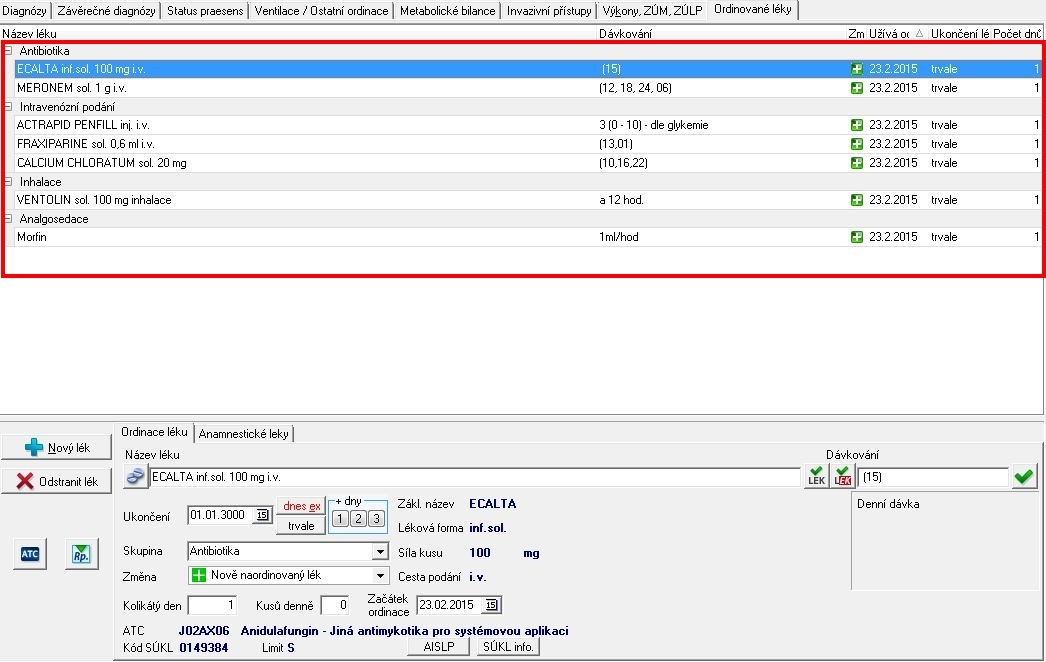
\includegraphics[width=1\textwidth]{img/medicalc/WM_ordinovane_leky.eps}
	\caption{Ordinované léky (WinMedicalc)}
  \label{fig:WM_ordinovane_leky}
\end{figure}

Medikační karta pro každého pacienta se poté vytiskne na papír do tabulky s vyznačenými hodinami. Tabulka nezačíná od půlnoci, ale od hodiny, kterou mají na oddělení nastavenou jako začátek dne (obvykle to bývá 6-7 hodina). Zdravotní sestry poté podle medikační karty podávají předepsané léky jednotlivým pacientům.

Způsoby zápisu ordinací se liší podle oddělení, ale i každá sestra má jiný styl zápisu. Vytištěné karty ordinovaných léků poté nemají jednotnou formu.

\subsection{Bilance tekutin}

V bilanci tekutin se zaznamenává příjem a výdej veškerých tekutin pacienta na lůžku i na operačním sále za celý den. Zaznamenává se 7 tekutin pro příjem a 5 tekutin pro výdej. Zároveň se počítá celkový příjem a celkový výdej všech tekutin. Rozložení jednotlivých tekutin je vidět na obrázku \ref{fig:WM_bilance_tekutin}.

\begin{figure}[H]
	\centering
	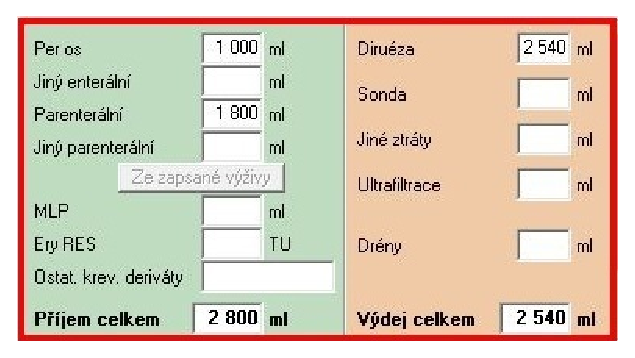
\includegraphics{img/medicalc/WM_bilance_tekutin.eps}
	\caption{Bilance tekutin (WinMedicalc)}
  \label{fig:WM_bilance_tekutin}
\end{figure}


Příjem a výdej tekutin odečítají zdravotní sestry během dne několikrát, ke každé tekutině tedy během dne bude několik hodnot. Všechny hodnoty se ukládají do databáze, aby bylo možné sledovat jejich vývoj.

Zdravotní sestry zaznamenávají příjem a výdej tekutin na papír. Na konci dne přepíší údaje do WinMedicalcu.

\subsection{Invazivní přístupy}

Pacient může mít zavedeno několik invazivních přístupů. Jedná se o katetry nebo drény. Každý invazivní přístup má vlastní specifikaci (číslo, název, umístění, hloubku zavedení, datum zavedení a počet dnů zavedení). Katetry a drény lze nechat v pacientovi zavedeny pouze po určitý počet dní (dle lékářských předpisů). Poté se musí vyměnit za nové nebo odebrat. Proto lze každý invazivní přístup v aplikaci označit požadavkem na výměnu. Následně jej lékař buď vymění, ve WinMedicalcu aktualizuje datum zavedení na datum výměny, nebo odebere a smaže ho ze seznamu invazivních přístupů. Změny invazivních přístupů do WinMedicalcu většinou zadává zdravotní sestra. Rozložení karty invazivních přístupů je na obrázku \ref{fig:WM_invazivni_pristupy}.

\begin{figure}[H]
	\centering
	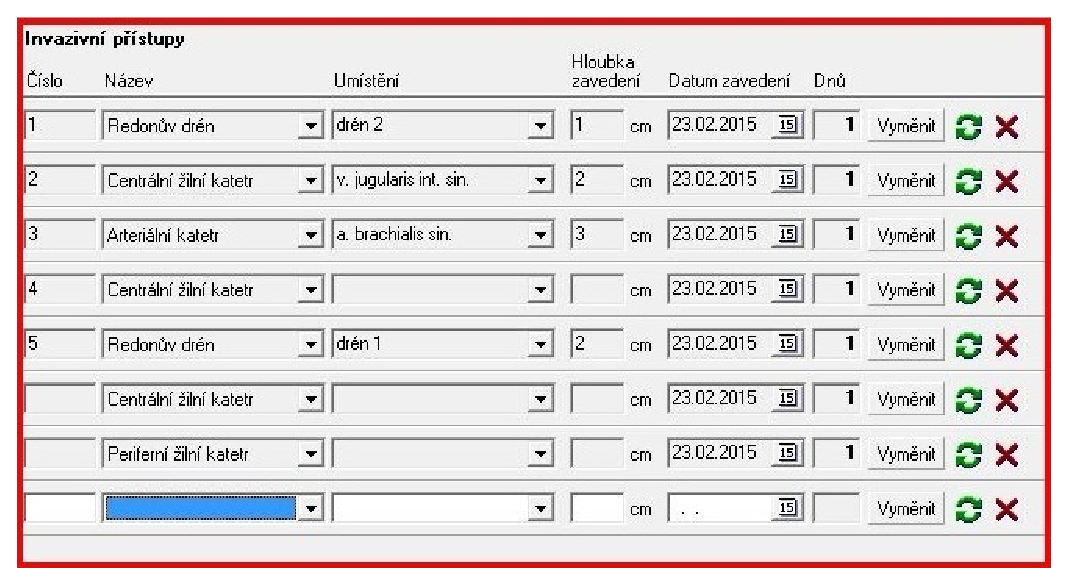
\includegraphics[width=1\textwidth]{img/medicalc/WM_invazivni_pristupy.eps}
	\caption{Invazivní přístupy (WinMedicalc)}
  \label{fig:WM_invazivni_pristupy}
\end{figure}


\subsection{Databáze}

Ve FN Plzeň je rozsáhlá databáze od Oraclu. V ní se ukládají prakticky všechny záznamy, včetně záznamů o pracovnících FN Plzeň, záznamů o pacientech a klinických událostech. Tato data se využijí ve vyvíjené aplikaci.

\section{Existující software}

Nemocničních informačních systémů existuje celá řada. Drtivá většina z nich jsou desktopové aplikace pro tablety naprosto nevhodné. Tyto softwary používají různé struktury pro ukládání dat. Také pořizovací náklady jsou vysoké, obvylášť proto, že se aplikace často musí upravit potřebám nemocnice.

Pro FN Plzeň, která se podílí na vývoji WinMedicalc a určuje strukturu dat, částečně splňoval požadavky jediný systém, ovšem za příliš vysoké pořizovací náklady. Proto se nemocnice rozhodla pro vývoj vlastího systému na míru, stejně, jako je tomu u WinMedicalcu.